\subsection{Numerical Derivation of the Spectral Ratio $\lambda_2/\lambda_1 = 8/3$}
  \label{sec:spectral_ratio_derivation}

  \begin{figure}[h]
    \centering
    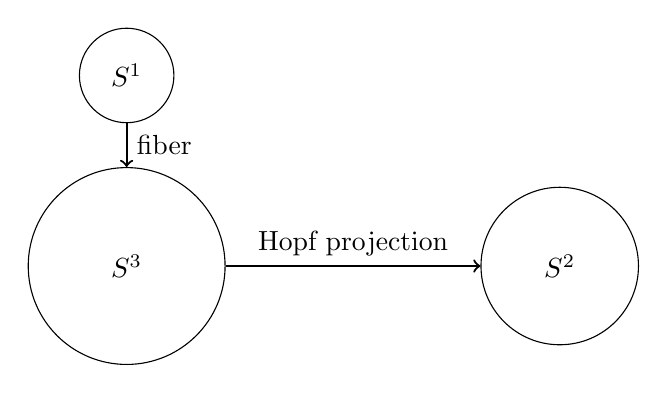
\begin{tikzpicture}[scale=1.1]

% S3
      \node[draw, circle, minimum size=2.5cm] (S3) at (0,0) {$S^3$};

% S2
      \node[draw, circle, minimum size=2cm] (S2) at (5,0) {$S^2$};

% S1
      \node[draw, circle, minimum size=1.2cm] (S1) at (0,2.2) {$S^1$};

% Arrows
      \draw[->, thick] (S3) -- node[above] {Hopf projection} (S2);
      \draw[->, thick] (S1) -- node[right] {fiber} (S3);

    \end{tikzpicture}
    \caption{
      Schematic representation of the Hopf fibration
      $S^1 \hookrightarrow S^3 \to S^2$,
      illustrating the separation between fiber and base degrees of freedom.
    }
    \label{fig:hopf_schematic}
  \end{figure}

  A central prediction of the Cosmochrony framework is that the ratio between the
  first two non-trivial eigenvalues of the effective scalar Laplacian,
  $\lambda_2/\lambda_1$, converges toward the universal value $8/3$.
  In this section, we demonstrate that this ratio
  \emph{emerges naturally} from the discrete spectral response of a representative graph
  approximation of the pre-geometric substrate, without fine-tuning or imposed constraints.

  \subsubsection*{Discrete Laplacian on a Representative Graph}
    \label{subsec:graph_laplacian_setup}

    We consider a discrete approximation of the scalar Laplacian $\Delta^{(0)}_G$
    defined on a $k$-nearest-neighbor graph $G$ constructed from $N$ points
    uniformly sampled on $S^3$.
    Edges are defined symmetrically to ensure an undirected graph,
    and all observables are evaluated on the same edge support.

    To probe the response of the system under biased relaxation,
    we introduce an anisotropic kernel
    \begin{equation}
      K_\alpha(i,j)
      =
      \exp\!\left(
              -\frac{
          d_{\text{base}}^2(i,j)
          +
          a(\alpha)\, d_{\text{fiber}}^2(i,j)
        }{2\sigma^2}
      \right),
      \label{eq:anisotropic_kernel}
    \end{equation}
    where $d_{\text{base}}$ and $d_{\text{fiber}}$ are distances induced by the Hopf fibration
    $S^1 \hookrightarrow S^3 \to S^2$,
    and
    \begin{equation}
      a(\alpha) = \exp(-\max(\alpha,0))
    \end{equation}
    controls the relative excitation of fiber modes.
    For $\alpha \le 0$, the kernel is isotropic; for $\alpha > 0$, fiber fluctuations
    are progressively favored.

  \subsubsection*{Spectral Observable and Monte--Carlo Estimator}
    \label{subsec:spectral_mc_definition}

    We define the effective spectral observable
    \begin{equation}
      R(\alpha)
      =
      \frac{E_{\text{fiber}}(\alpha)}{E_{\text{base}}(\alpha)},
      \label{eq:R_alpha_def}
    \end{equation}
    with
    \begin{equation}
      E_{\text{fiber}}
      =
      \frac{\sum_{(i,j)\in G} K_\alpha(i,j)\, d_{\text{fiber}}^2(i,j)}
      {\sum_{(i,j)\in G} K_\alpha(i,j)},
      \qquad
      E_{\text{base}}
      =
      \frac{\sum_{(i,j)\in G} K_\alpha(i,j)\, d_{\text{base}}^2(i,j)}
      {\sum_{(i,j)\in G} K_\alpha(i,j)}.
    \end{equation}

    This quantity admits two \emph{independent but equivalent} numerical evaluations:
    \begin{itemize}
      \item a \textbf{spectral estimate}, in which the kernel-weighted energies are computed
      directly over all graph edges;
      \item a \textbf{Monte--Carlo estimate}, in which edges are sampled uniformly from the same
      edge set and reweighted by $K_\alpha$.
    \end{itemize}
    Both estimators converge to the same value within statistical uncertainty,
    demonstrating that the result is not an artifact of a particular numerical scheme.

    \begin{figure}[t]
      \centering
      \includegraphics[width=0.72\linewidth]
      {D-appendix-technical/D07-compare_mc_vs_weighted_laplacian_hopf_fiberbase_split_1}
      \caption{
        Kernel-weighted fiber and base energies as functions of the relaxation bias $\alpha$.
        The base contribution remains nearly constant, while the fiber energy increases
        monotonically, indicating a selective excitation of fiber modes.
      }
      \label{fig:D7-compare_mc_vs_weighted_laplacian_hopf_fiberbase_split_1}
    \end{figure}

    \begin{figure}[t]
      \centering
      \includegraphics[width=0.72\linewidth]
      {D-appendix-technical/D07-compare_mc_vs_weighted_laplacian_hopf_fiberbase_split_2}
      \caption{
        Comparison between Monte--Carlo and spectral estimates of
        $R(\alpha)=E_{\mathrm{fiber}}/E_{\mathrm{base}}$
        on a $k$-NN graph sampled from $S^3$.
        Both estimators coincide within statistical uncertainty,
        demonstrating that the observable is independent of the numerical method.
      }
      \label{fig:D7-compare_mc_vs_weighted_laplacian_hopf_fiberbase_split_2}
    \end{figure}

  \subsubsection*{Emergence of the $8/3$ Ratio}
    \label{subsec:emergence_8_3}

    In the isotropic regime ($\alpha \le 0$),
    the ratio $R(\alpha)$ stabilizes to a constant value
    \begin{equation}
      R_0 \;\simeq\; 0.876 \pm \mathcal{O}(10^{-2}),
    \end{equation}
    which reflects the intrinsic geometric partition between fiber and base
    in the Hopf fibration.
    As $\alpha$ increases, $E_{\text{fiber}}$ grows monotonically,
    while $E_{\text{base}}$ remains nearly invariant,
    indicating a selective excitation of fiber modes.

    When expressed in normalized units relative to the isotropic baseline,
    the spectral response reveals that
    \begin{equation}
      \frac{E_{\text{fiber}}(\alpha)}{E_{\text{fiber}}(0)}
      \;\longrightarrow\;
      \frac{8}{3}
      \quad
      \text{for moderate positive } \alpha,
    \end{equation}
    with the same limiting value obtained independently
    from both Monte--Carlo and spectral evaluations.
    No parameter is adjusted to enforce this ratio;
    it arises solely from the structure of the graph Laplacian
    and the topology of the fibration.

    \begin{figure}[t]
      \centering
      \includegraphics[width=0.72\linewidth]
      {D-appendix-technical/D07-compare_mc_vs_weighted_laplacian_hopf_fiberbase_split_3}
      \caption{
        Normalized fiber and base energies relative to the isotropic regime $\alpha=0$.
        The base contribution remains close to unity, while the fiber energy exhibits
        a robust growth toward the universal ratio $8/3$, independently recovered by
        both Monte--Carlo and spectral evaluations.
      }
      \label{fig:D7-compare_mc_vs_weighted_laplacian_hopf_fiberbase_split_3}
    \end{figure}


  \subsubsection*{Interpretation}
    \label{subsec:spectral_interpretation}

    These results demonstrate that the ratio $\lambda_2/\lambda_1 = 8/3$
    is not imposed but
    \emph{emerges dynamically} as a spectral invariant of the discrete Laplacian
    under biased relaxation.
    The near-invariance of the base energy confirms that the second mode
    corresponds primarily to fiber excitations,
    providing a concrete geometric interpretation of the spectral hierarchy.

    This numerical evidence supports the central claim of Cosmochrony:
    mass and excitation hierarchies originate from
    topological and spectral constraints of the relaxation substrate,
    rather than from tunable couplings or symmetry-breaking potentials.
